%\newpage
\section{Modeling uncertainty of ISRF near the GC} 
\lb{app:ISRF}

In this appendix we discuss the uncertainty of the IC model of the gamma-ray emission at the base of the FBs 
related to modeling of the ISRF near the GC.
In order to estimate this uncertainty, we compare the GALPROP v54.1 model of ISRF
\citep{2006ApJ...640L.155M,  2006ApJ...648L..29P},
the ISRF model of \cite{2017MNRAS.470.2539P}%
\footnote{We would like to thank Cristina Popescu for providing us the ISRF data files in fits format.},
and two ISRF models of \cite{2017ApJ...846...67P}: 
R12, based on \cite{2012A&A...545A..39R},
and F98, based on \cite{1998ApJ...492..495F}.
The corresponding densities of ISRFs at the GC are shown in Figure \ref{fig:isrfs}.
We notice that there can be up to two orders of magnitude differences in the ISRF energy densities,
which can affect the inferred populations of CR electrons producing the IC gamma rays 
\citep[see also][]{2017ApJ...846...67P, 2019APh...107....1N}.

\begin{figure*}[h]
\centering
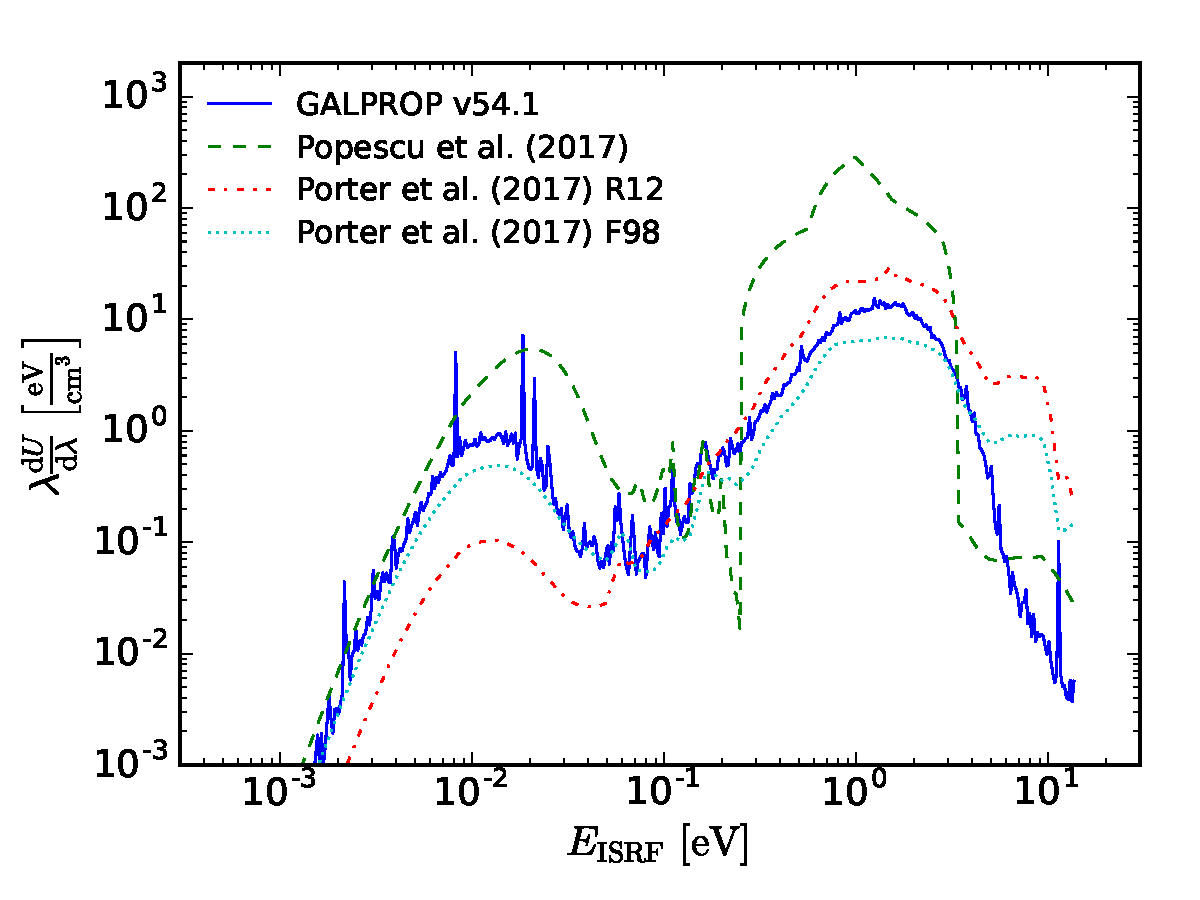
\includegraphics[width=\twopic\textwidth]{plots/ISRF_comparison}
\caption{Comparison of ISRF SEDs at the GC (see text for more details).}
\label{fig:isrfs}
\end{figure*}

In Figure \ref{fig:GC_CR} we show the IC models of the gamma-ray emission 
at the base of the FBs in the rectangle $b \in (-2\degr, 2\degr)$, $\ell \in (-10\degr, 0\degr)$
for the different ISRF models near the GC.
We separate the starlight (SL), infrared (IR) and cosmic microwave background (CMB) contributions.
The SL and IR ISRFs are separated by splitting the radiation field energy densities at 0.1 eV.
We model the CR electrons spectra by power-law function with an exponential cutoff.
We fix the cutoff at 1 PeV and fit the normalization and the spectral index by fitting 
the IC model to the \Fermi-LAT spectral points.
The corresponding parameters are presented in Table \ref{tab:CRe_syst}.
We use the GALPROP v54.1 ISRF as the reference model and show the normalizations of the CRe spectra
relative to the reference model (the normalizations are determined at 1 GeV).
The overall spread in the normalizations is about factor of 30,
while the variation of the index of the CRe spectra is less than 0.15.

\begin{figure*}[h]
\centering
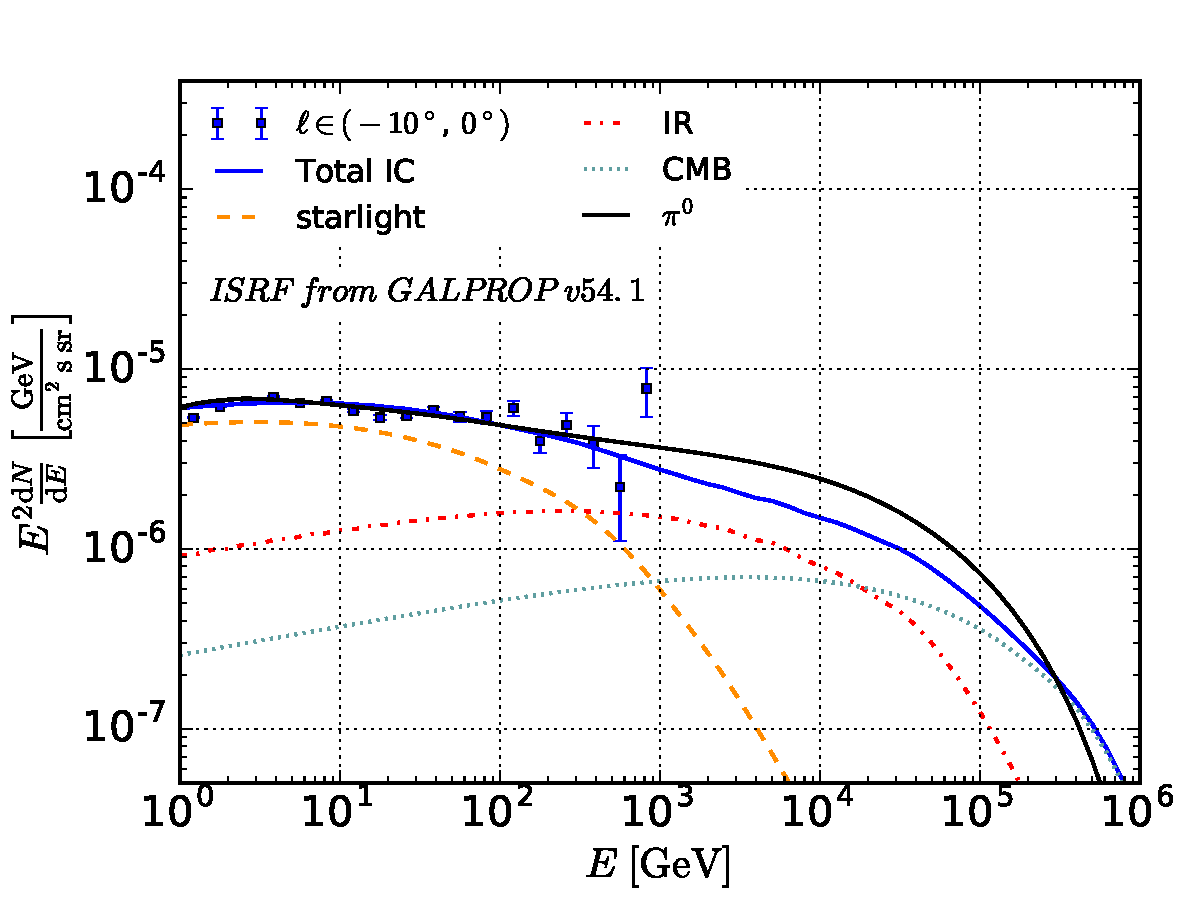
\includegraphics[width=\twopic\textwidth]{plots/SED_ISRF_componentsboxes_source_0_v54}
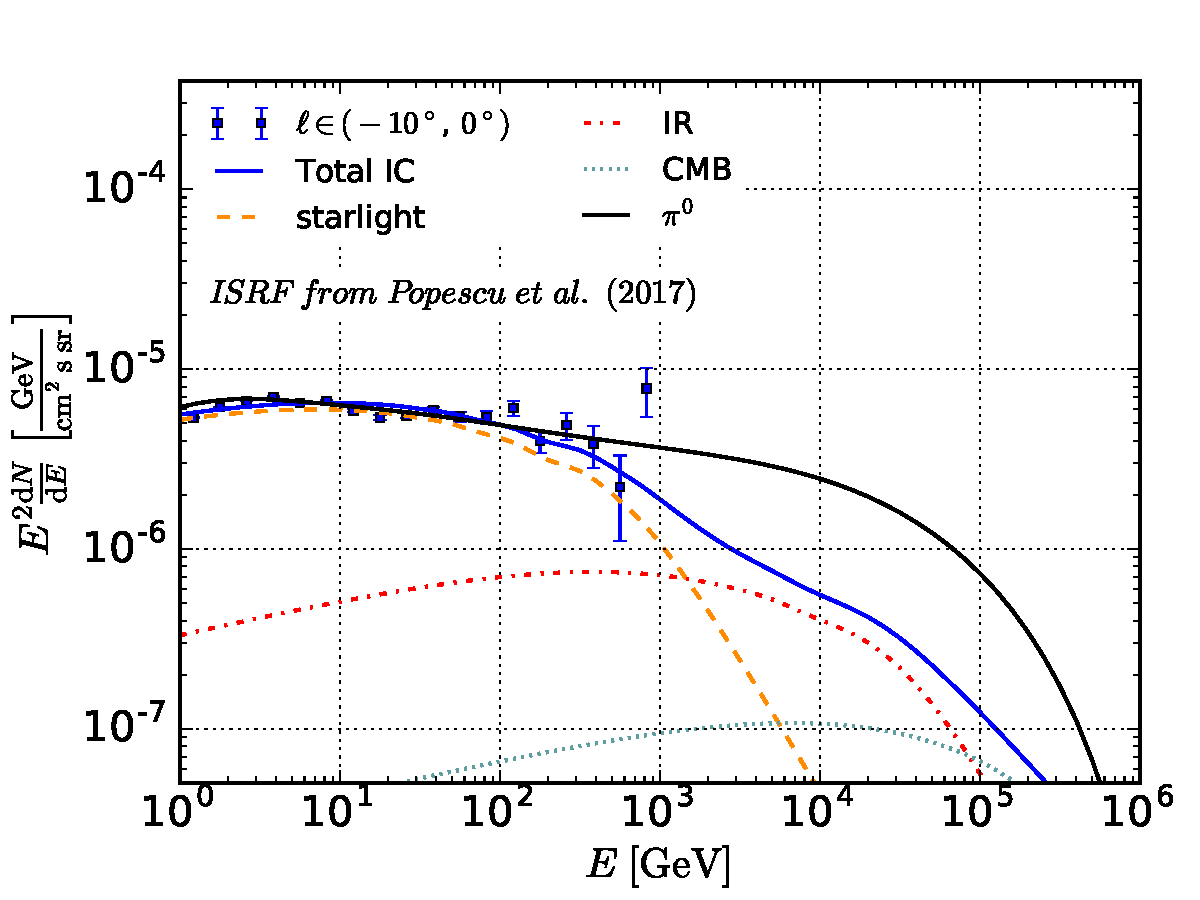
\includegraphics[width=\twopic\textwidth]{plots/SED_ISRF_componentsboxes_source_0_Popescu}
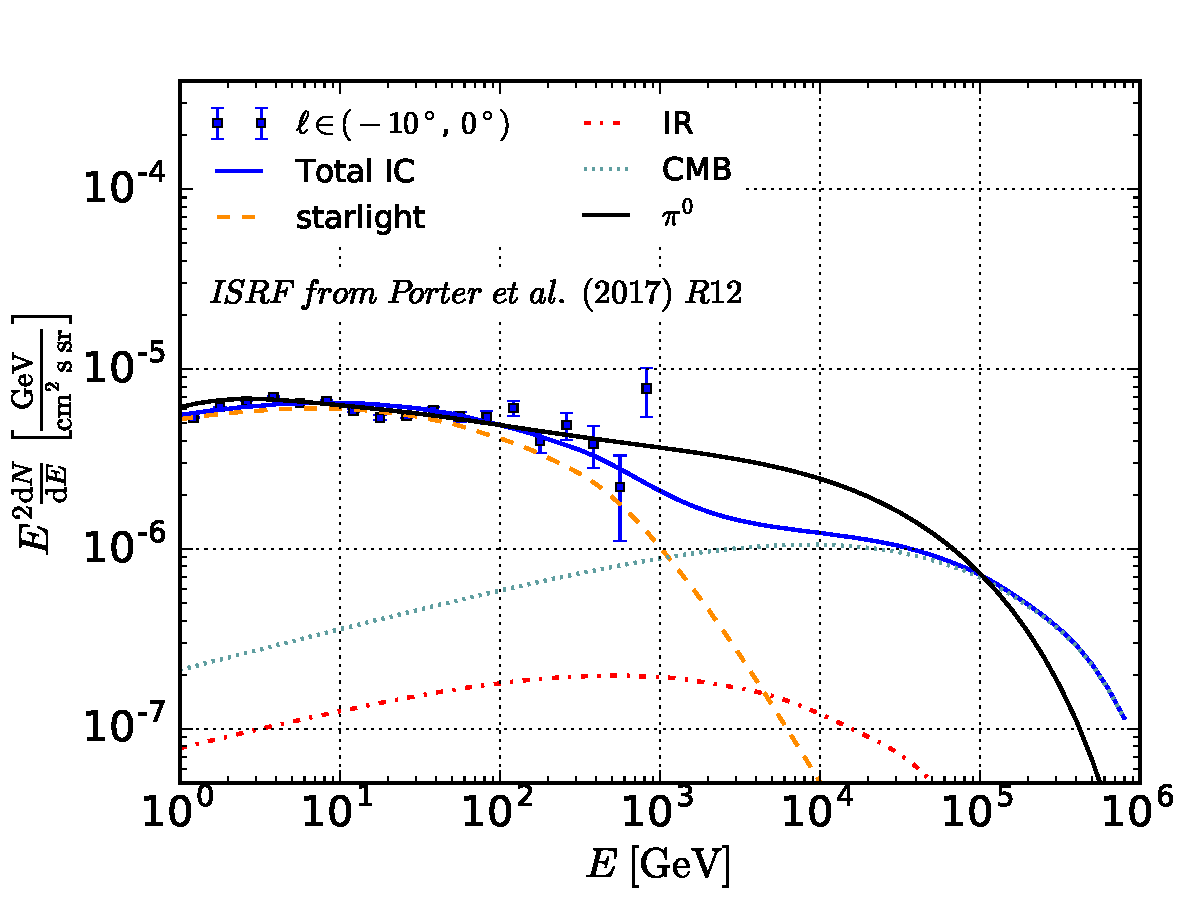
\includegraphics[width=\twopic\textwidth]{plots/SED_ISRF_componentsboxes_source_0_R12}
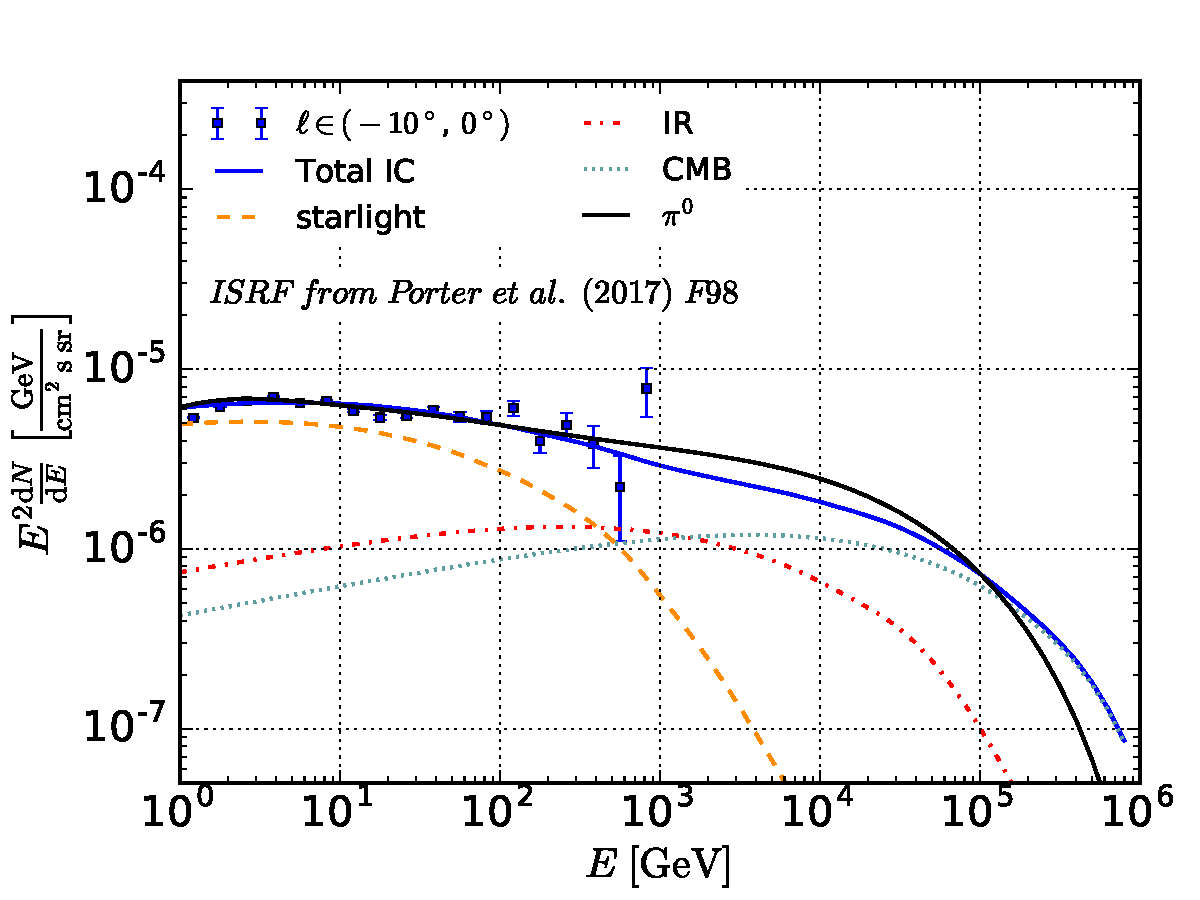
\includegraphics[width=\twopic\textwidth]{plots/SED_ISRF_componentsboxes_source_0_F98}
\caption{Contribution of different components of ISRFs to the IC model of the gamma-ray emission.
The data points correspond to the emission at the base of the FBs in the rectangle $b \in (-2\degr, 2\degr)$, $\ell \in (-10\degr, 0\degr)$
(middle panel in Figure \ref{fig:SED_with_fits}).
The spectrum of CR electrons is modeled by a power-law function with an exponential  cutoff at 1 PeV.
We separate the starlight and the IR contributions to the ISRF by formally splitting the ISRF at 0.1 eV.
The CR proton spectrum in the $\pi^0$ model of the gamma-ray emission
is modeled a power-law function with an exponential cutoff at 1 PeV.}
\label{fig:GC_CR}
\end{figure*}

\begin{table*}
  \begin{center}
    \caption{\label{tab:CRe_syst} 
Spectra of CR electrons near the GC relative to the reference model based on GALPROP v54.1 ISRF.
}
    \begin{tabular}{| l |c|c|} % <-- Alignments: 1st column left, 2nd middle and 3rd right, with vertical lines in between
     	\hline
		 ISRF model & Relative normalization at 1 GeV  & Index \\
		\hline
  		GALPROP v54.1 & 1 & 1.67 \\ 
  		\cite{2017ApJ...846...67P} R12 & 0.36 & 1.54 \\ 
  		\cite{2017ApJ...846...67P} F98 & 1.6 & 1.67 \\ 
  		\cite{2017MNRAS.470.2539P} & 0.057 & 1.58 \\ 
 \hline
    \end{tabular}
  \end{center}
\end{table*}



